


%----------------------------------
\chapter{Introduction}\label{ch:Eulerintro}
%----------------------------------

\section{Purpose and Objectives of the \EulerDescT}
%%%%%%%%%%%%%%%%%%%%%%%%%%%%%%%%%%%%%%%%%%%%%%%%%%%%%%%%%%%%%%%%%%%%%%%%%%%%%%%%%
%
% Purpose:  Introduction for the Euler model.
%
% 
%
%%%%%%%%%%%%%%%%%%%%%%%%%%%%%%%%%%%%%%%%%%%%%%%%%%%%%%%%%%%%%%%%%%%%%%%%%%%%%%%%


%\section{Purpose and Objectives of \EulerDesc}
% Incorporate the intro paragraph that used to begin this Chapter here. 
% This is location of the true introduction where you explain what this model 
% does.
The Euler Derived State represents the relative attitude of a particular reference frame with respect to some other frame as a series of Euler angle rotations.  The output will be a 3-vector of angles; the user may specify in which order those angles are to be expressed.

















%----------------------------------
\chapter{Product Requirements}\label{ch:Eulerreqt}
%----------------------------------


%%%%%%%%%%%%%%%%%%%%%%%%%%%%%%%%%%%%%%%%%%%%%%%%%%%%%%%%%%%%%%%%%%%%%%%%%%%%%%%%%
%
% Purpose:  requirements for the Euler model
%
% 
%
%%%%%%%%%%%%%%%%%%%%%%%%%%%%%%%%%%%%%%%%%%%%%%%%%%%%%%%%%%%%%%%%%%%%%%%%%%%%%%%%

% add text here to describe general model requirements
% text is of the form:
\requirement{Calculate relative attitude between two reference frames}
\label{reqt:Euler}
\begin{description}
  \item[Requirement:]\ \newline
     Given a reference frame associated with a body, the \EulerDesc\ will calculate an Euler-type angle sequence from body frame to the reference frame parent to it, and from the parent frame to the body frame using the 3 basic axes, represented as roll(x-axis rotation), pitch (y-axis rotation), and yaw (z-axis rotation).
  \item[Rationale:]\ \newline
     To provide a means of expressing relative attitude between reference frames.
  \item[Verification:]\ \newline
     Test
\end{description}

\section{Requirements Traceability}

\begin{longtable}[c]{||p{3.5in}|p{3.5in}|}
\caption{Requirements Traceability} \\[6pt]
\hline
{\bf Requirement} & {\bf Inspection and Testing} \\ 
\hline \hline
\endhead
\ref{reqt:Euler} - Calculate relative attitude between two reference frames &
  Test~\ref{test:Euler} \\ \hline
\end{longtable}




%----------------------------------
\chapter{Product Specification}\label{ch:Eulerspec}
%----------------------------------

\section{Conceptual Design}
%%%%%%%%%%%%%%%%%%%%%%%%%%%%%%%%%%%%%%%%%%%%%%%%%%%%%%%%%%%%%%%%%%%%%%%%%%%%%%%%%
%
% Purpose:  Conceptual part of Product Spec for the Euler model
%
% 
%
%%%%%%%%%%%%%%%%%%%%%%%%%%%%%%%%%%%%%%%%%%%%%%%%%%%%%%%%%%%%%%%%%%%%%%%%%%%%%%%%


%\section{Conceptual Design}
A reference frame attitude can be described as a set of three rotations about independent axes.  In the \EulerDesc\, the Roll, Pitch, and Yaw axes are used, and can be input in any order \textbf{without repeats} (i.e. all three axes must be used).  Numerically, three values are specified in a single vector, corresponding to the angle of rotation about each specified axis in turn.

The angles represent a process for conducting a transformation from one reference frame to another, thereby providing data on the relative attitude of the two frames.  Because the relative attitude can be expressed in either direction, two sets of angles, \textit{ref\_body\_angles} and \textit{body\_ref\_angles} are included in the available output.  \textit{ref\_body\_angles} provides the transformation from the external reference frame to the subject-body reference frame, and \textit{body\_ref\_angles} provides the reverse transformation.

When calculating the Euler angles from two reference frames, both sets of angles are calculated.

%\section{Mathematical Formulations}
%%%%%%%%%%%%%%%%%%%%%%%%%%%%%%%%%%%%%%%%%%%%%%%%%%%%%%%%%%%%%%%%%%%%%%%%%%%%%%%%%
%
% Purpose:  Mathematical Formulation part of Product Spec for the Euler model
%
% 
%
%%%%%%%%%%%%%%%%%%%%%%%%%%%%%%%%%%%%%%%%%%%%%%%%%%%%%%%%%%%%%%%%%%%%%%%%%%%%%%%%

\section{Mathematical Formulations}
The \EulerDesc\ relies on the Trick method \textit{euler\_matrix} for generating the euler angles.  No further mathematical framework is implemented in the \EulerDesc.
%\section{Detailed Design}

%%%%%%%%%%%%%%%%%%%%%%%%%%%%%%%%%%%%%%%%%%%%%%%%%%%%%%%%%%%%%%%%%%%%%%%%%%%%%%%%%
%
% Purpose:  Detailed part of Product Spec for the Euler model
%
% 
%
%%%%%%%%%%%%%%%%%%%%%%%%%%%%%%%%%%%%%%%%%%%%%%%%%%%%%%%%%%%%%%%%%%%%%%%%%%%%%%%%

\section{Detailed Design}

See the \href{file:refman.pdf}{Reference Manual}\cite{derivedstatebib:ReferenceManual} for a summary of member data and member methods for all classes.  

\subsection{Process Architecture}
The process architecture for the \EulerDesc\ is trivial, comprising entirely independent methods.

\subsection{Functional Design}
This section describes the functional operation of the methods in each class.

The \EulerDesc\ contains only one class:
\begin{itemize}
\classitem{EulerDerivedState}
\textref{DerivedState}{ref:DerivedState}

This contains the methods \textit{initialize}, and \textit{update}:
\begin{enumerate}

\funcitem{initialize}
There are two processes for initialization, depending on the relationship in the Reference Frame Tree between the subject-body reference frame, and the exterior reference frame.  If the former is not a child of the latter, then it becomes necessary to specify which frame is to be used as the external reference frame.  In this case, a separate initialization process allows for the specification of that frame.  Otherwise, the initialization process simply calls the generic DerivedState initialization routine to establish the naming convention of the reference object (i.e., the planet about which the vehicle is orbiting) and state identifier.

\funcitem{update}
If the Euler angles are to be computed relative to a frame other than the parent frame, that relative state is first calculated.  Then the Trick method \textit{euler\_matrix} is called for both reference-to-subject and subject-to-reference frame transformations.

\end{enumerate}
\end{itemize}


\chapter{User's Guide}\label{ch:Euleruser}
%----------------------------------
The Analysis section of the User's Guide is intended primarily for
users of pre-existing simulations.  
It contains: 
\begin{itemize}
\item A description of how to modify \EulerDesc\ variables after
the simulation
has compiled, including an in-depth discussion of the input file,
\item An overview of how to interpret (but not edit) the S\_define
file,
\item A sample of some of the typical variables that may be logged.
\end{itemize}

The Integration section of the User's Guide is intended for simulation
developers.
It describes the necessary configuration of the \EulerDesc\
within an
S\_define file, and the creation of standard run directories.  The
latter
component assumes a thorough understanding of the preceding Analysis
section of the user guide.
Where applicable, the user may be directed to selected portions of
Product Specification (Chapter \ref{ch:Eulerspec}).

The Extension section of the User's Guide is intended primarily for
developers
needing to extend the capability of the \EulerDesc.  Such users
should have a
thorough understanding of how the model is used in the preceding
Integration section, and of the model
specification (described in Chapter \ref{ch:Eulerspec}).


\section{Analysis}
%%%%%%%%%%%%%%%%%%%%%%%%%%%%%%%%%%%%%%%%%%%%%%%%%%%%%%%%%%%%%%%%%%%%%%%%%%%%%%%%%
%
% Purpose:  Analysis part of User's Guide for the Euler model
%
% 
%
%%%%%%%%%%%%%%%%%%%%%%%%%%%%%%%%%%%%%%%%%%%%%%%%%%%%%%%%%%%%%%%%%%%%%%%%%%%%%%%%

% \section{Analysis}

\label{sec:euleruseranalysis}
\subsection{Identifying the \EulerDescT}
If the Euler angles have been included in the simulation, there will be an instance of \textit{EulerDerivedState} located in the S\_define file.  This would typically be found in the vehicle object.  There should be an accompanying call to an initialization routine, which takes a reference to the \textit{subject\_body} as one if its inputs, and may also take a reference to a reference-frame, although this is not necessary.  There will also be an accompanying call to an update function.  The essential variable \textit{sequence}, the order in which the angles should be assigned to each axis, is defined elsewhere, often in the input file.

Example:
\begin{verbatim}
sim_object{
dynamics/derived_state:    EulerDerivedState example_of_euler_angles;

(initialization) dynamics/derived_state:
example_of_rel_state_object.example_of_euler_angles.initialize (
    Inout DynBody &      subject_body = vehicle_1.dyn_body,
    Inout DynManager &   dyn_manager  = manager_object.dyn_manager);
    
{environment} dynamics/derived_state:
example_of_rel_state_object.example_of_euler_angles.update ( )

} example_of_rel_state_object;
\end{verbatim}

The input file may contain an entry comparable to:
\begin{verbatim}
example_of_rel_state_object.example_of_euler_angles.sequence = Roll_Pitch_Yaw;
\end{verbatim}
This variable can take one of the following values:
\begin{itemize}
\item{} Roll\_ Pitch\_ Yaw
\item{} Roll\_ Yaw\_ Pitch
\item{} Pitch\_ Yaw\_ Roll
\item{} Pitch\_ Roll\_ Yaw
\item{} Yaw\_ Roll\_ Pitch
\item{} Yaw\_ Pitch\_ Roll
\end{itemize}

\subsection{Editing the \EulerDescT}
The sequence is open to edit by the analyst.

\subsection{Output Data}
The direct output from the \EulerDesc\ comprises only the two vectors of angles,
\textit{ref\_body\_angles} (the Euler angles from the reference frame to the subject frame), and
\textit{body\_ref\_angles} (the Euler angles to the reference frame from the subject frame).
\begin{verbatim}
example_of_rel_state_object.example_of_euler_angles.ref_body_angles[0-2]
example_of_rel_state_object.example_of_euler_angles.body_ref_angles[0-2]
\end{verbatim}





%\section{Integration}
%%%%%%%%%%%%%%%%%%%%%%%%%%%%%%%%%%%%%%%%%%%%%%%%%%%%%%%%%%%%%%%%%%%%%%%%%%%%%%%%%
%
% Purpose:  Integration part of User's Guide for the Euler model
%
% 
%
%%%%%%%%%%%%%%%%%%%%%%%%%%%%%%%%%%%%%%%%%%%%%%%%%%%%%%%%%%%%%%%%%%%%%%%%%%%%%%%%

 \section{Integration}
Simply including the \EulerDesc\ is a trivial undertaking, all of the contents that can be included into the model are identified in the previous section (\ref{sec:euleruseranalysis}).

%\section{Extension}
%%%%%%%%%%%%%%%%%%%%%%%%%%%%%%%%%%%%%%%%%%%%%%%%%%%%%%%%%%%%%%%%%%%%%%%%%%%%%%%%%
%
% Purpose:  Extension part of User's Guide for the Euler model
%
% 
%
%%%%%%%%%%%%%%%%%%%%%%%%%%%%%%%%%%%%%%%%%%%%%%%%%%%%%%%%%%%%%%%%%%%%%%%%%%%%%%%%

 \section{Extension}
The \EulerDesc\ is not written with the intention of being extended.

%----------------------------------
\chapter{Verification and
Validation}\label{ch:Eulerivv}
%----------------------------------

\section{Verification}
%%%%%%%%%%%%%%%%%%%%%%%%%%%%%%%%%%%%%%%%%%%%%%%%%%%%%%%%%%%%%%%%%%%%%%%%%%%%%%%%%
%
% Purpose:  Verification part of V&V for the Euler model
%
% 
%
%%%%%%%%%%%%%%%%%%%%%%%%%%%%%%%%%%%%%%%%%%%%%%%%%%%%%%%%%%%%%%%%%%%%%%%%%%%%%%%%

% \section{Verification}

%%% code imported from old template structure
%\inspection{<Name of Inspection>}\label{inspect:<label>}
% <description> to satisfy  
% requirement \ref{reqt:<label>}.

 For testing the \EulerDesc\, a single vehicle was initialized in one of 3 orbits: an equatorial circular orbit, an inclined orbit, and an eccentric equatorial orbit.  An LVLH frame was also generated, and the Euler angles between the vehicle body frame (the subject frame), and the LVLH frame (the reference frame), were computed.  

\test{Verification of \EulerDesc\ Output Data}\label{test:Euler}

\begin{description}
\item{Purpose:}\newline
To demonstrate that the output from the \EulerDesc\ provides meaningful data.

\item{Requirements:}\newline
Satisfactory conclusion of this test satisfies requirement \ref{reqt:Euler}

\item{Procedure:}\newline
Two cases were considered, one in which the vehicle frame was initially aligned with the LVLH frame, and one in which it was given an initial relative attitude.  In both cases, the vehicle body frame was initialized with no rotation (with respect to the inertial frame).  Since the LVLH frame maintains an orientation dependent upon the position of the origin, the two frames rotate with respect to one another.  The angles generated by this orbital motion are considered.

\item{Predictions:}  
In the LVLH frame, the frame-to-frame relative rotation will appear as a pitch (rotation about the LVLH y-axis).  In the tests in which the two frames are initially aligned, that is equivalent to a pitch in the body frame.  Both transformations should exhibit slowly oscillating pitch values, with constant zero values for yaw and roll.

When the two frames are not initially aligned, in general, the variation of angles resulting from the varying relative attitude will be across all three axes.  Exceptions to this rule include transformations from body to LVLH that end with a pitch, or those from LVLH to body that start with a pitch.  This is due to the order of calculation, consider the transformation from body to LVLH:

The transformation from body to initial LVLH frame is constant, and the LVLH rotates with respect to the initial LVLH frame on its y-axis; a transformation from body to LVLH can be seen as a combination of transformations from body to the initial LVLH frame followed by one from the initial LVLH frame to LVLH, which comprises only a pitch component.  Therefore, if pitch is last in the order, the two pitch adjustments simply add; the roll and yaw are due to the constant difference between body and initial LVLH, and so should remain constant, whereas the pitch should start at some pre-assigned value, and exhibit the same periodic variation thereafter that was seen in the case of the initially aligned frames.  The same argument can be traced in reverse for the reverse transformation.

For other sets in which the pitch is calculated in an inconvenient sequence (second or third, or first from body frame to reference frame, or last in reference frame to body frame), the effect in the yaw and roll angles of the addition of the pitch due to the variational relative frame rotation will manifest as a time dependency on all 3 axes, due to the cross-coupling effects of rotational sequences.

The variation with time in the rate at which the angles change will be constant for the circular orbits, but variable for the elliptic orbits.

For further confirmation of the data, the euler angles of the vehicle with respect to the inertially-oriented planetary axes we investigated, these should show no variation.

\item{Results:}
All output data confirmed expectations, within numerical precision.  Some expected constant values were not quite constant, but exhibited some very small oscillatory or noisy behavior.  

For the aligned frames, the YRP, RYP, PYR, and PRY sequences showed the pitch slowly changing  from $\pm \pi$ to $\mp \pi$ before immediately resetting.  The YPR and RPY sequences had the pitch varying only between $\pm \frac{\pi}{2}$, and doing so with constant ramps up and down.  For these two sequences, the roll and pitch also switched to $\pm \pi$ during the time that the pitch was decreasing, and returned to zero while the pitch was increasing.  These solutions are completely valid, and illustrate that there is more than one way to represent a particular orientation.  These results were valid for both the LVLH-body and body-LVLH orientations. See figures~\ref{fig:euleralignedpyr} and~\ref{fig:euleralignedrpy} for Pitch-Yaw-Roll and Roll-Pitch-Yaw sequences.

\begin{figure}[!ht]
\begin{center}
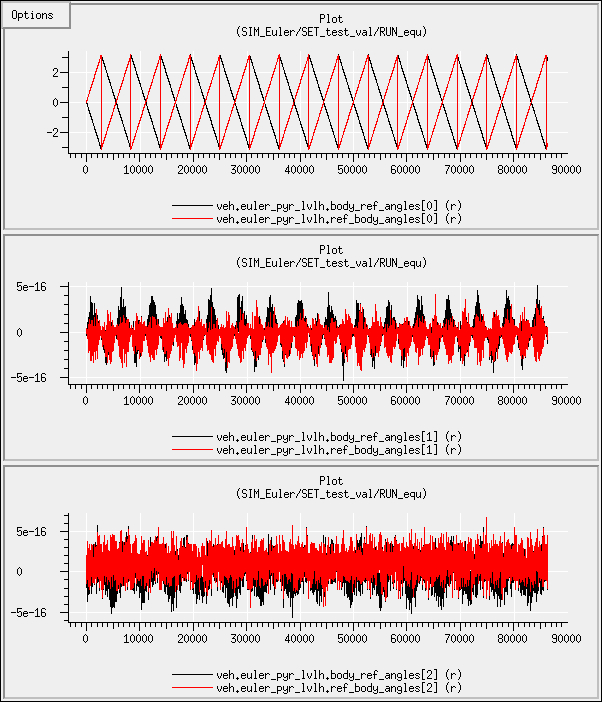
\includegraphics[width=5in]{figures/euler_aligned_pyr.jpg}
\caption{The Euler angles for the case in which the LVLH frame and body frame were initially aligned, and rotating with respect to each other on their respective pitch axes, expressed in a Pitch-Yaw-Roll sequence.}
\label{fig:euleralignedpyr}
\end{center}
\end{figure}

\begin{figure}[!ht]
\begin{center}
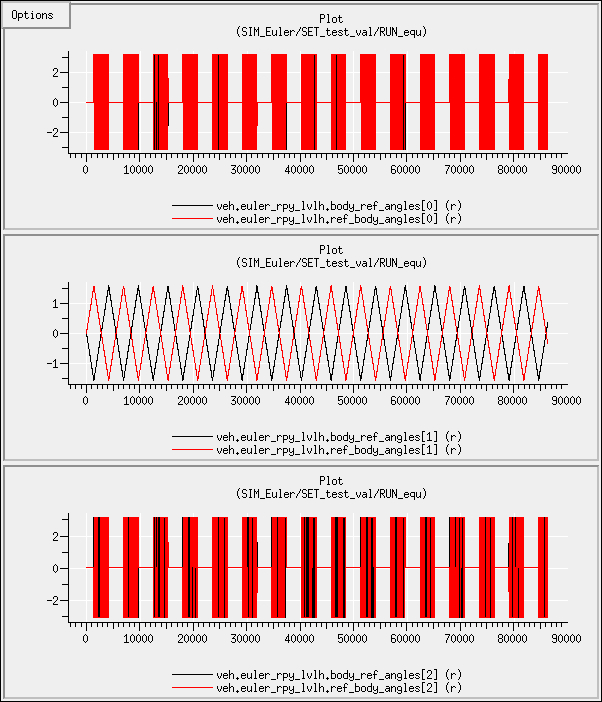
\includegraphics[width=5in]{figures/euler_aligned_rpy.jpg}
\caption{The Euler angles for the case in which the LVLH frame and body frame were initially aligned, and rotating with respect to each other on their respective pitch axes, expressed in a Roll-Pitch-Yaw sequence.  Notice that the Pitch has a total range of only $\pi$ radians; this is compensated for by the combined effect of adding in $\pi$ rotations on the yaw and roll axes.}
\label{fig:euleralignedrpy}
\end{center}
\end{figure}

For the tests in which the frames were not initially aligned, those with Pitch in the correct sequencing showed the similar pattern to the aligned frames, as expected.  Other sequences had periodic behavior.  See Figures~\ref{fig:eulernonalignedpyr},~\ref{fig:eulernonalignedrpy}, and~\ref{fig:eulernonalignedyrp} for Pitch-Yaw-Roll, Roll-Pitch-Yaw, and Yaw-Roll-Pitch sequences.

\begin{figure}[!ht]
\begin{center}
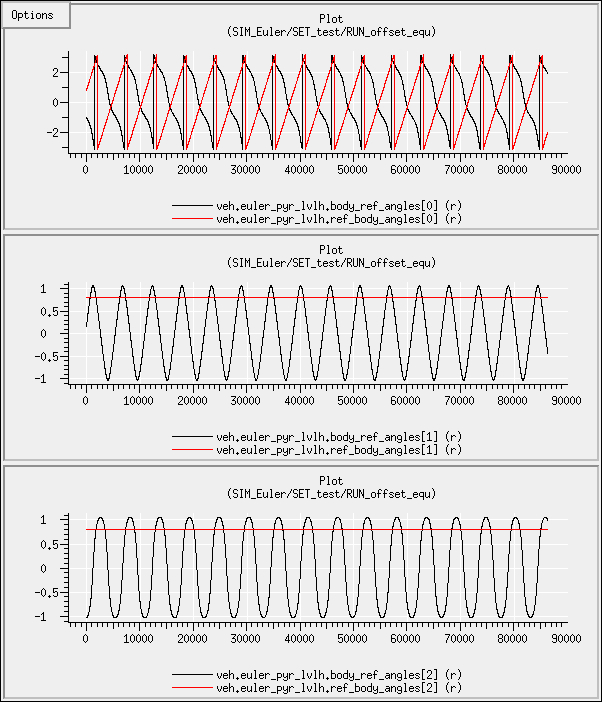
\includegraphics[width=5in]{figures/euler_nonaligned_pyr.jpg}
\caption{The Euler angles for the case in which the LVLH frame and body frame were initially un-aligned, and rotating with respect to each other on the pitch axis of the LVLH reference frame.  Angles are expressed in a Pitch-Yaw-Roll sequence.  Notice that when Pitch is first in the sequence, the angles associated with the transformation from the LVLH frame to the body frame (expressed in the LVLH frame) show a similar pattern to that in Figure~\ref{fig:euleralignedpyr}, but that is not the case when representing the relative attitude from the body frame to the LVLH frame (this is expressed in the body frame).}
\label{fig:eulernonalignedpyr}
\end{center}
\end{figure}

\begin{figure}[!ht]
\begin{center}
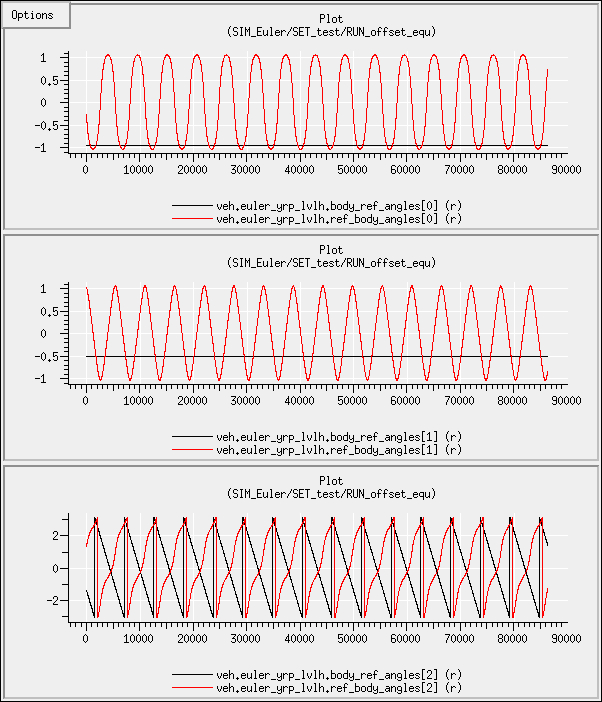
\includegraphics[width=5in]{figures/euler_nonaligned_yrp.jpg}
\caption{The Euler angles for the case in which the LVLH frame and body frame were initially un-aligned, and rotating with respect to each other on the pitch axis of the LVLH reference frame.  Angles are expressed in a Yaw-Roll-Pitch sequence.  Notice that when Pitch is last in the sequence, the angles associated with the transformation from body frame to LVLH (expressed in body frame) show a similar pattern to that in Figure~\ref{fig:euleralignedpyr}, but that is not the case when representing the relative attitude from the LVLH frame to the body frame (this is expressed in the LVLH frame).}
\label{fig:eulernonalignedyrp}
\end{center}
\end{figure}

\begin{figure}[!ht]
\begin{center}
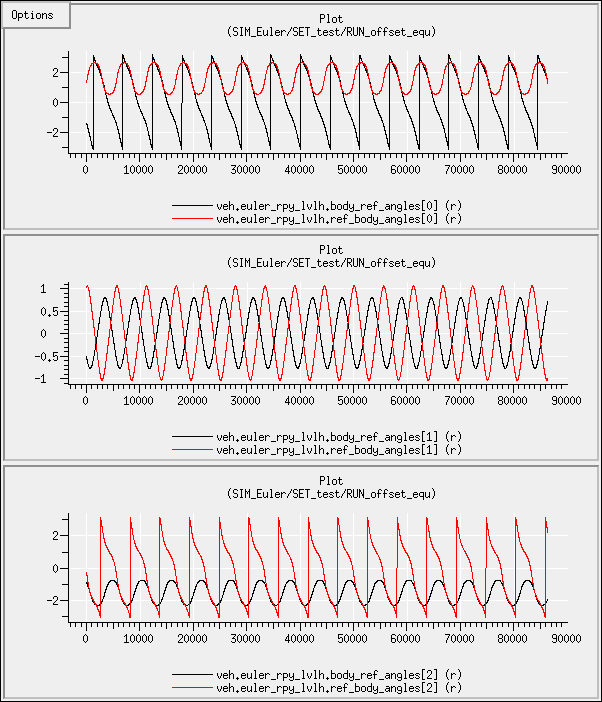
\includegraphics[width=5in]{figures/euler_nonaligned_rpy.jpg}
\caption{The Euler angles for the case in which the LVLH frame and body frame were initially un-aligned, and rotating with respect to each other on the pitch axis of the LVLH reference frame.  Notice that the variation is non-sinusoidal, and that the amplitudes differ between the two representations of the transformation.}
\label{fig:eulernonalignedrpy}
\end{center}
\end{figure}




\end{description}


%\section{Validation}
%%%%%%%%%%%%%%%%%%%%%%%%%%%%%%%%%%%%%%%%%%%%%%%%%%%%%%%%%%%%%%%%%%%%%%%%%%%%%%%%%
%
% Purpose:  Validation part of V&V for the Euler model
%
% 
%
%%%%%%%%%%%%%%%%%%%%%%%%%%%%%%%%%%%%%%%%%%%%%%%%%%%%%%%%%%%%%%%%%%%%%%%%%%%%%%%%

\section{Validation}

There is no independent validation of this sub-model.
%%% code imported from old template structure
%\test{<Title>}\label{test:<label>}
%\begin{description}
%\item[Purpose:] \ \newline
%<description>
%\item[Requirements:] \ \newline
%By passing this test, the universal time module 
%partially satisfies requirement~\ref{reqt:<label1>} and 
%completely satisfies requirement~\ref{reqt:<label2>}.
%\item[Procedure:]\ \newline
%<procedure>
%\item[Results:]\ \newline
%<results>
%\end{description}




